\documentclass[output=paper,
modfonts
]{LSP/langsci}


%% add all extra packages you need to load to this file 
% \usepackage{todo} %% removed,cna use todonotes instead. % Jason reactivated
% \usepackage{graphicx} % not needed because forest loads tikz, which loads graphicx
\usepackage{tabularx}
\usepackage{amsmath} 
\usepackage{multicol}
\usepackage{lipsum}
\usepackage{longtable}
\usepackage{booktabs}
\usepackage[normalem]{ulem}
%\usepackage{tikz} % not needed because forest loads tikz
\usepackage{phonrule} % for SPE-style phonological rules
\usepackage{pst-all} % loads the main pstricks tools; for arrow diagrams in Hale.tex
%\usepackage{leipzig} % for gloss abbreviations
\usepackage[% for automatic cross-referencing
compress,%
capitalize,% labels are always capitalized in LSP style
noabbrev]% labels are always spelled out in LSP style
{cleveref}

% based on http://tex.stackexchange.com/a/318983/42880 for using gb4e examples with cleveref
\crefname{xnumi}{}{}
\creflabelformat{xnumi}{(#2#1#3)}
\crefrangeformat{xnumi}{(#3#1#4)--(#5#2#6)}
\crefname{xnumii}{}{}
\creflabelformat{xnumii}{(#2#1#3)}
\crefrangeformat{xnumii}{(#3#1#4)--(#5#2#6)}

%\usepackage[notcite,notref]{showkeys} %%removed, not helping CB.
%\usepackage{showidx} %%remove for final compiling - shows index keys at top of page.
 
\usepackage{langsci/styles/langsci-gb4e}  
 \usepackage{pifont}
% % OT tableaux                                                
% \usepackage{pstricks,colortab}  
\usepackage{multirow} % used in OT tableaux
\usepackage{rotating} %needed for angled text%
\usepackage{colortbl} % for cell shading
 
 \usepackage{avm}  
\usepackage[linguistics]{forest} 
\usetikzlibrary{matrix,fit} % for matrix of nodes in Kaisse and Bat-El


\usepackage{hhline}
\newcommand{\cgr}{\cellcolor[gray]{0.8}}
\newcommand{\cn}{\centering}



\newcommand{\reff}[1]{(\ref{#1})}
%\usepackage{newtxtext,newtxmath}


%\usepackage[normalem] {ulem}
\usepackage{qtree}
%\usepackage{natbib}
%\usepackage{tikz}
%\usepackage{gb4e}
\usepackage{phonrule}  
%\bibliographystyle{humannat}



\usepackage{minibox}

%\include{psheader-metr}

\def\bl#1{$_{\textrm{{\footnotesize #1}}}$}

%%add all your local new commands to this file

\newcommand{\form}[1]{\mbox{\emph{#1}}}
\newcommand{\uf}[1]{\mbox{/#1/}}

% borrowed from expex and converted from plan tex to latex
\newcommand{\judge}[1]{{\upshape #1\hspace{0.1em}}}
\newcommand{\ljudge}[1]{\makebox[0pt][r]{\judge{#1}}}

\newcommand\tikzmark[1]{\tikz[remember picture, baseline=(#1.base)] \node[anchor=base,inner sep=0pt, outer sep=0pt] (#1) {#1};} % for adding decorations, arrows, lines, etc. to text
\newcommand\tikzmarknamed[2]{\tikz[remember picture, baseline=(#1.base)] \node[anchor=base,inner sep=0pt, outer sep=0pt] (#1) {#2};} % for adding decorations, arrows, lines, etc. to text
\newcommand\tikzmarkfullnamed[2]{\tikz[remember picture, baseline=(#1.base)] \node[anchor=base,inner sep=0pt, outer sep=0pt] (#1) {\vphantom{X}#2};} % for adding decorations, arrows, lines, etc. to text; this one works best for decorations above a line of text because it adds in the heigh of a capital letter and takes two arguments - one for the node name and one for the printed text

\newcommand{\sub}[1]{$_{\text{#1}}$} % for non-math subscripts
\newcommand{\subit}[1]{\sub{\textit{#1}}} % for italics non-math subscripts
\newcommand{\1}{\rlap{$'$}\xspace} % for the prime in X' (the \rlap command allows the prime to be ignored for horizontal spacing in trees, and the \xspace command allows you to use this in normal text without adding \ afterwards). This isn't crucial, but it helps the formatting to look a little better.

% Aissen:
\newcommand\tikzmarkfull[1]{\tikz[remember picture, baseline=(#1.base)] \node[anchor=base,inner sep=0pt, outer sep=0pt] (#1) {\vphantom{X}#1};} % for adding decorations, arrows, lines, etc. to text; this one works best for decorations above a line of text because it adds in the heigh of a capital letter and takes one argument that serves as the name and the printed text
\newcommand{\bridgeover}[2]{% for a line that creates a bridge over text, connecting two nodes
	\begin{tikzpicture}[remember picture,overlay]
	\draw[thick,shorten >=3pt,shorten <=3pt] (#1.north) |- +(0ex,2.5ex) -| (#2.north);
	\end{tikzpicture}
}
\newcommand{\bridgeoverht}[3]{% for a line that creates a bridge over text, connecting two nodes and specifing the height of the bridge
	\begin{tikzpicture}[remember picture,overlay]
	\draw[thick,shorten >=3pt,shorten <=3pt] (#2.north) |- +(0ex,#1) -| (#3.north);
	\end{tikzpicture}
}
\newcommand{\bridgeoverex}{\vspace*{3ex}} % place before an example that has a \bridgeover so that there is enough vertical space for it

% Chung:
\newcommand{\lefttabular}[1]{\begin{tabular}{p{0.5in}}#1\end{tabular}}

% Kaisse:
\newcommand{\mgmorph}[1]{|(#1)| {#1}}
\newcommand{\mgone}[2][$\times$]{\node at (#2.base) [above=2ex] (1#2) {\vphantom{X}#1};}
\newcommand{\mgtwo}[2][$\times$]{\mgone{#2} \node at (#2.base) [above=4.5ex] (2#2) {\vphantom{X}#1};}
\newcommand{\mgthree}[2][$\times$]{\mgtwo{#2} \node at (#2.base) [above=7ex] (3#2) {\vphantom{X}#1};}
\newcommand{\mgftl}[1]{\node at (1#1) [left] {(};}
\newcommand{\mgftr}[1]{\node at (1#1) [right] {)};}
\newcommand{\mgfoot}[2]{\mgftl{#1}\mgftr{#2}}
\newcommand{\mgldelim}[2]{\node at (#2.west) [left,inner sep = 0pt, outer sep = 0pt] {#1};}
\newcommand{\mgrdelim}[2]{\node at (#2.east) [right,inner sep = 0pt, outer sep = 0pt] {#1};}

\newcommand{\squish}{\hspace*{-3pt}}

% Kavitskaya:
\newcommand{\assoc}[2]{\draw (#1.south) -- (#2.north);}
\newcolumntype{L}{>{\raggedright\arraybackslash}X}

% Lepic & Padden:
\newcommand{\fitpic}[1]{\resizebox{\hsize}{!}{\includegraphics{#1}}} % from http://tex.stackexchange.com/a/148965/42880
\newcommand{\signpic}[1]{\includegraphics[width=1.36in]{#1}}
\newcolumntype{C}{>{\centering\arraybackslash}X}

% Spencer:

\newcommand{\textex}[1]{\textit{#1}\xspace}
\newcommand{\lxm}[1]{\textsc{#1}\xspace}

% Thrainsson:

\renewcommand{\textasciitilde}{\char`~} % for use with TTF/OTF fonts (see comments on http://tex.stackexchange.com/a/317/42880)
\newcommand{\tikzarrow}[2]{% for an arrow connecting two nodes
\begin{tikzpicture}[remember picture,overlay]
\draw[thick,shorten >=3pt,shorten <=3pt,->,>=stealth] (#1) -- (#2);
\end{tikzpicture}
}

\newlength{\padding}
\setlength{\padding}{0.5em}
\newcommand{\lesspadding}{\hspace*{-\padding}}
\newcommand{\feat}[1]{\lesspadding#1\lesspadding}

% Hammond

\usepackage[]{graphicx}\usepackage[]{xcolor}
%% maxwidth is the original width if it is less than linewidth
%% otherwise use linewidth (to make sure the graphics do not exceed the margin)
\makeatletter
\def\maxwidth{ %
  \ifdim\Gin@nat@width>\linewidth
    \linewidth
  \else
    \Gin@nat@width
  \fi
}
\makeatother

\definecolor{fgcolor}{rgb}{0.345, 0.345, 0.345}
\newcommand{\hlnum}[1]{\textcolor[rgb]{0.686,0.059,0.569}{#1}}%
\newcommand{\hlstr}[1]{\textcolor[rgb]{0.192,0.494,0.8}{#1}}%
\newcommand{\hlcom}[1]{\textcolor[rgb]{0.678,0.584,0.686}{\textit{#1}}}%
\newcommand{\hlopt}[1]{\textcolor[rgb]{0,0,0}{#1}}%
\newcommand{\hlstd}[1]{\textcolor[rgb]{0.345,0.345,0.345}{#1}}%
\newcommand{\hlkwa}[1]{\textcolor[rgb]{0.161,0.373,0.58}{\textbf{#1}}}%
\newcommand{\hlkwb}[1]{\textcolor[rgb]{0.69,0.353,0.396}{#1}}%
\newcommand{\hlkwc}[1]{\textcolor[rgb]{0.333,0.667,0.333}{#1}}%
\newcommand{\hlkwd}[1]{\textcolor[rgb]{0.737,0.353,0.396}{\textbf{#1}}}%
\let\hlipl\hlkwb

\usepackage{framed}
\makeatletter
\newenvironment{kframe}{%
 \def\at@end@of@kframe{}%
 \ifinner\ifhmode%
  \def\at@end@of@kframe{\end{minipage}}%
  \begin{minipage}{\columnwidth}%
 \fi\fi%
 \def\FrameCommand##1{\hskip\@totalleftmargin \hskip-\fboxsep
 \colorbox{shadecolor}{##1}\hskip-\fboxsep
     % There is no \\@totalrightmargin, so:
     \hskip-\linewidth \hskip-\@totalleftmargin \hskip\columnwidth}%
 \MakeFramed {\advance\hsize-\width
   \@totalleftmargin\z@ \linewidth\hsize
   \@setminipage}}%
 {\par\unskip\endMakeFramed%
 \at@end@of@kframe}
\makeatother

\definecolor{shadecolor}{rgb}{.97, .97, .97}
\definecolor{messagecolor}{rgb}{0, 0, 0}
\definecolor{warningcolor}{rgb}{1, 0, 1}
\definecolor{errorcolor}{rgb}{1, 0, 0}
\newenvironment{knitrout}{}{} % an empty environment to be redefined in TeX

\usepackage{alltt}

%revised version started: 12/17/16

%NEEDS: allbib.bib - already added to the master bibliography file.
%cited references only: bibexport -o mhTMP.bib main1-blx.aux
%PLUS sramh-img*, sramh.tex

%added stuff
\newcommand{\add}[1]{\textcolor{blue}{#1}}
%deleted stuff
\newcommand{\del}[1]{\textcolor{red}{(removed: #1)}}
%uncomment these to turn off colors
\renewcommand{\add}[1]{#1}
\renewcommand{\del}[1]{}

%shortcuts
\newcommand{\w}{\ili{Welsh}}
\newcommand{\e}{\ili{English}}
\newcommand{\io}{Input Optimization}




 \newcommand{\hand}{\ding{43}}
% \newcommand{\rot}[1]{\begin{rotate}{90}#1\end{rotate}} %shortcut for angled text%  
% \newcommand{\rotcon}[1]{\raisebox{-5ex}{\hspace*{1ex}\rot{\hspace*{1ex}#1}}}

%% add all extra packages you need to load to this file 
% \usepackage{todo} %% removed,cna use todonotes instead. % Jason reactivated
% \usepackage{graphicx} % not needed because forest loads tikz, which loads graphicx
\usepackage{tabularx}
\usepackage{amsmath} 
\usepackage{multicol}
\usepackage{lipsum}
\usepackage{longtable}
\usepackage{booktabs}
\usepackage[normalem]{ulem}
%\usepackage{tikz} % not needed because forest loads tikz
\usepackage{phonrule} % for SPE-style phonological rules
\usepackage{pst-all} % loads the main pstricks tools; for arrow diagrams in Hale.tex
%\usepackage{leipzig} % for gloss abbreviations
\usepackage[% for automatic cross-referencing
compress,%
capitalize,% labels are always capitalized in LSP style
noabbrev]% labels are always spelled out in LSP style
{cleveref}

% based on http://tex.stackexchange.com/a/318983/42880 for using gb4e examples with cleveref
\crefname{xnumi}{}{}
\creflabelformat{xnumi}{(#2#1#3)}
\crefrangeformat{xnumi}{(#3#1#4)--(#5#2#6)}
\crefname{xnumii}{}{}
\creflabelformat{xnumii}{(#2#1#3)}
\crefrangeformat{xnumii}{(#3#1#4)--(#5#2#6)}

%\usepackage[notcite,notref]{showkeys} %%removed, not helping CB.
%\usepackage{showidx} %%remove for final compiling - shows index keys at top of page.
 
\usepackage{langsci/styles/langsci-gb4e}  
 \usepackage{pifont}
% % OT tableaux                                                
% \usepackage{pstricks,colortab}  
\usepackage{multirow} % used in OT tableaux
\usepackage{rotating} %needed for angled text%
\usepackage{colortbl} % for cell shading
 
 \usepackage{avm}  
\usepackage[linguistics]{forest} 
\usetikzlibrary{matrix,fit} % for matrix of nodes in Kaisse and Bat-El


\usepackage{hhline}
\newcommand{\cgr}{\cellcolor[gray]{0.8}}
\newcommand{\cn}{\centering}



\newcommand{\reff}[1]{(\ref{#1})}
%\usepackage{newtxtext,newtxmath}


%\usepackage[normalem] {ulem}
\usepackage{qtree}
%\usepackage{natbib}
%\usepackage{tikz}
%\usepackage{gb4e}
\usepackage{phonrule}  
%\bibliographystyle{humannat}



\usepackage{minibox}

%\include{psheader-metr}

\def\bl#1{$_{\textrm{{\footnotesize #1}}}$}
\usepackage{arydshln}
\usepackage{rotating}

%%add all your local new commands to this file

\newcommand{\form}[1]{\mbox{\emph{#1}}}
\newcommand{\uf}[1]{\mbox{/#1/}}

% borrowed from expex and converted from plan tex to latex
\newcommand{\judge}[1]{{\upshape #1\hspace{0.1em}}}
\newcommand{\ljudge}[1]{\makebox[0pt][r]{\judge{#1}}}

\newcommand\tikzmark[1]{\tikz[remember picture, baseline=(#1.base)] \node[anchor=base,inner sep=0pt, outer sep=0pt] (#1) {#1};} % for adding decorations, arrows, lines, etc. to text
\newcommand\tikzmarknamed[2]{\tikz[remember picture, baseline=(#1.base)] \node[anchor=base,inner sep=0pt, outer sep=0pt] (#1) {#2};} % for adding decorations, arrows, lines, etc. to text
\newcommand\tikzmarkfullnamed[2]{\tikz[remember picture, baseline=(#1.base)] \node[anchor=base,inner sep=0pt, outer sep=0pt] (#1) {\vphantom{X}#2};} % for adding decorations, arrows, lines, etc. to text; this one works best for decorations above a line of text because it adds in the heigh of a capital letter and takes two arguments - one for the node name and one for the printed text

\newcommand{\sub}[1]{$_{\text{#1}}$} % for non-math subscripts
\newcommand{\subit}[1]{\sub{\textit{#1}}} % for italics non-math subscripts
\newcommand{\1}{\rlap{$'$}\xspace} % for the prime in X' (the \rlap command allows the prime to be ignored for horizontal spacing in trees, and the \xspace command allows you to use this in normal text without adding \ afterwards). This isn't crucial, but it helps the formatting to look a little better.

% Aissen:
\newcommand\tikzmarkfull[1]{\tikz[remember picture, baseline=(#1.base)] \node[anchor=base,inner sep=0pt, outer sep=0pt] (#1) {\vphantom{X}#1};} % for adding decorations, arrows, lines, etc. to text; this one works best for decorations above a line of text because it adds in the heigh of a capital letter and takes one argument that serves as the name and the printed text
\newcommand{\bridgeover}[2]{% for a line that creates a bridge over text, connecting two nodes
	\begin{tikzpicture}[remember picture,overlay]
	\draw[thick,shorten >=3pt,shorten <=3pt] (#1.north) |- +(0ex,2.5ex) -| (#2.north);
	\end{tikzpicture}
}
\newcommand{\bridgeoverht}[3]{% for a line that creates a bridge over text, connecting two nodes and specifing the height of the bridge
	\begin{tikzpicture}[remember picture,overlay]
	\draw[thick,shorten >=3pt,shorten <=3pt] (#2.north) |- +(0ex,#1) -| (#3.north);
	\end{tikzpicture}
}
\newcommand{\bridgeoverex}{\vspace*{3ex}} % place before an example that has a \bridgeover so that there is enough vertical space for it

% Chung:
\newcommand{\lefttabular}[1]{\begin{tabular}{p{0.5in}}#1\end{tabular}}

% Kaisse:
\newcommand{\mgmorph}[1]{|(#1)| {#1}}
\newcommand{\mgone}[2][$\times$]{\node at (#2.base) [above=2ex] (1#2) {\vphantom{X}#1};}
\newcommand{\mgtwo}[2][$\times$]{\mgone{#2} \node at (#2.base) [above=4.5ex] (2#2) {\vphantom{X}#1};}
\newcommand{\mgthree}[2][$\times$]{\mgtwo{#2} \node at (#2.base) [above=7ex] (3#2) {\vphantom{X}#1};}
\newcommand{\mgftl}[1]{\node at (1#1) [left] {(};}
\newcommand{\mgftr}[1]{\node at (1#1) [right] {)};}
\newcommand{\mgfoot}[2]{\mgftl{#1}\mgftr{#2}}
\newcommand{\mgldelim}[2]{\node at (#2.west) [left,inner sep = 0pt, outer sep = 0pt] {#1};}
\newcommand{\mgrdelim}[2]{\node at (#2.east) [right,inner sep = 0pt, outer sep = 0pt] {#1};}

\newcommand{\squish}{\hspace*{-3pt}}

% Kavitskaya:
\newcommand{\assoc}[2]{\draw (#1.south) -- (#2.north);}
\newcolumntype{L}{>{\raggedright\arraybackslash}X}

% Lepic & Padden:
\newcommand{\fitpic}[1]{\resizebox{\hsize}{!}{\includegraphics{#1}}} % from http://tex.stackexchange.com/a/148965/42880
\newcommand{\signpic}[1]{\includegraphics[width=1.36in]{#1}}
\newcolumntype{C}{>{\centering\arraybackslash}X}

% Spencer:

\newcommand{\textex}[1]{\textit{#1}\xspace}
\newcommand{\lxm}[1]{\textsc{#1}\xspace}

% Thrainsson:

\renewcommand{\textasciitilde}{\char`~} % for use with TTF/OTF fonts (see comments on http://tex.stackexchange.com/a/317/42880)
\newcommand{\tikzarrow}[2]{% for an arrow connecting two nodes
\begin{tikzpicture}[remember picture,overlay]
\draw[thick,shorten >=3pt,shorten <=3pt,->,>=stealth] (#1) -- (#2);
\end{tikzpicture}
}

\newlength{\padding}
\setlength{\padding}{0.5em}
\newcommand{\lesspadding}{\hspace*{-\padding}}
\newcommand{\feat}[1]{\lesspadding#1\lesspadding}

% Hammond

\usepackage[]{graphicx}\usepackage[]{xcolor}
%% maxwidth is the original width if it is less than linewidth
%% otherwise use linewidth (to make sure the graphics do not exceed the margin)
\makeatletter
\def\maxwidth{ %
  \ifdim\Gin@nat@width>\linewidth
    \linewidth
  \else
    \Gin@nat@width
  \fi
}
\makeatother

\definecolor{fgcolor}{rgb}{0.345, 0.345, 0.345}
\newcommand{\hlnum}[1]{\textcolor[rgb]{0.686,0.059,0.569}{#1}}%
\newcommand{\hlstr}[1]{\textcolor[rgb]{0.192,0.494,0.8}{#1}}%
\newcommand{\hlcom}[1]{\textcolor[rgb]{0.678,0.584,0.686}{\textit{#1}}}%
\newcommand{\hlopt}[1]{\textcolor[rgb]{0,0,0}{#1}}%
\newcommand{\hlstd}[1]{\textcolor[rgb]{0.345,0.345,0.345}{#1}}%
\newcommand{\hlkwa}[1]{\textcolor[rgb]{0.161,0.373,0.58}{\textbf{#1}}}%
\newcommand{\hlkwb}[1]{\textcolor[rgb]{0.69,0.353,0.396}{#1}}%
\newcommand{\hlkwc}[1]{\textcolor[rgb]{0.333,0.667,0.333}{#1}}%
\newcommand{\hlkwd}[1]{\textcolor[rgb]{0.737,0.353,0.396}{\textbf{#1}}}%
\let\hlipl\hlkwb

\usepackage{framed}
\makeatletter
\newenvironment{kframe}{%
 \def\at@end@of@kframe{}%
 \ifinner\ifhmode%
  \def\at@end@of@kframe{\end{minipage}}%
  \begin{minipage}{\columnwidth}%
 \fi\fi%
 \def\FrameCommand##1{\hskip\@totalleftmargin \hskip-\fboxsep
 \colorbox{shadecolor}{##1}\hskip-\fboxsep
     % There is no \\@totalrightmargin, so:
     \hskip-\linewidth \hskip-\@totalleftmargin \hskip\columnwidth}%
 \MakeFramed {\advance\hsize-\width
   \@totalleftmargin\z@ \linewidth\hsize
   \@setminipage}}%
 {\par\unskip\endMakeFramed%
 \at@end@of@kframe}
\makeatother

\definecolor{shadecolor}{rgb}{.97, .97, .97}
\definecolor{messagecolor}{rgb}{0, 0, 0}
\definecolor{warningcolor}{rgb}{1, 0, 1}
\definecolor{errorcolor}{rgb}{1, 0, 0}
\newenvironment{knitrout}{}{} % an empty environment to be redefined in TeX

\usepackage{alltt}

%revised version started: 12/17/16

%NEEDS: allbib.bib - already added to the master bibliography file.
%cited references only: bibexport -o mhTMP.bib main1-blx.aux
%PLUS sramh-img*, sramh.tex

%added stuff
\newcommand{\add}[1]{\textcolor{blue}{#1}}
%deleted stuff
\newcommand{\del}[1]{\textcolor{red}{(removed: #1)}}
%uncomment these to turn off colors
\renewcommand{\add}[1]{#1}
\renewcommand{\del}[1]{}

%shortcuts
\newcommand{\w}{\ili{Welsh}}
\newcommand{\e}{\ili{English}}
\newcommand{\io}{Input Optimization}




 \newcommand{\hand}{\ding{43}}
% \newcommand{\rot}[1]{\begin{rotate}{90}#1\end{rotate}} %shortcut for angled text%  
% \newcommand{\rotcon}[1]{\raisebox{-5ex}{\hspace*{1ex}\rot{\hspace*{1ex}#1}}}

%% add all extra packages you need to load to this file 
% \usepackage{todo} %% removed,cna use todonotes instead. % Jason reactivated
% \usepackage{graphicx} % not needed because forest loads tikz, which loads graphicx
\usepackage{tabularx}
\usepackage{amsmath} 
\usepackage{multicol}
\usepackage{lipsum}
\usepackage{longtable}
\usepackage{booktabs}
\usepackage[normalem]{ulem}
%\usepackage{tikz} % not needed because forest loads tikz
\usepackage{phonrule} % for SPE-style phonological rules
\usepackage{pst-all} % loads the main pstricks tools; for arrow diagrams in Hale.tex
%\usepackage{leipzig} % for gloss abbreviations
\usepackage[% for automatic cross-referencing
compress,%
capitalize,% labels are always capitalized in LSP style
noabbrev]% labels are always spelled out in LSP style
{cleveref}

% based on http://tex.stackexchange.com/a/318983/42880 for using gb4e examples with cleveref
\crefname{xnumi}{}{}
\creflabelformat{xnumi}{(#2#1#3)}
\crefrangeformat{xnumi}{(#3#1#4)--(#5#2#6)}
\crefname{xnumii}{}{}
\creflabelformat{xnumii}{(#2#1#3)}
\crefrangeformat{xnumii}{(#3#1#4)--(#5#2#6)}

%\usepackage[notcite,notref]{showkeys} %%removed, not helping CB.
%\usepackage{showidx} %%remove for final compiling - shows index keys at top of page.
 
\usepackage{langsci/styles/langsci-gb4e}  
 \usepackage{pifont}
% % OT tableaux                                                
% \usepackage{pstricks,colortab}  
\usepackage{multirow} % used in OT tableaux
\usepackage{rotating} %needed for angled text%
\usepackage{colortbl} % for cell shading
 
 \usepackage{avm}  
\usepackage[linguistics]{forest} 
\usetikzlibrary{matrix,fit} % for matrix of nodes in Kaisse and Bat-El


\usepackage{hhline}
\newcommand{\cgr}{\cellcolor[gray]{0.8}}
\newcommand{\cn}{\centering}



\newcommand{\reff}[1]{(\ref{#1})}
%\usepackage{newtxtext,newtxmath}


%\usepackage[normalem] {ulem}
\usepackage{qtree}
%\usepackage{natbib}
%\usepackage{tikz}
%\usepackage{gb4e}
\usepackage{phonrule}  
%\bibliographystyle{humannat}



\usepackage{minibox}

%\include{psheader-metr}

\def\bl#1{$_{\textrm{{\footnotesize #1}}}$}
\usepackage{arydshln}
\usepackage{rotating}

%%add all your local new commands to this file

\newcommand{\form}[1]{\mbox{\emph{#1}}}
\newcommand{\uf}[1]{\mbox{/#1/}}

% borrowed from expex and converted from plan tex to latex
\newcommand{\judge}[1]{{\upshape #1\hspace{0.1em}}}
\newcommand{\ljudge}[1]{\makebox[0pt][r]{\judge{#1}}}

\newcommand\tikzmark[1]{\tikz[remember picture, baseline=(#1.base)] \node[anchor=base,inner sep=0pt, outer sep=0pt] (#1) {#1};} % for adding decorations, arrows, lines, etc. to text
\newcommand\tikzmarknamed[2]{\tikz[remember picture, baseline=(#1.base)] \node[anchor=base,inner sep=0pt, outer sep=0pt] (#1) {#2};} % for adding decorations, arrows, lines, etc. to text
\newcommand\tikzmarkfullnamed[2]{\tikz[remember picture, baseline=(#1.base)] \node[anchor=base,inner sep=0pt, outer sep=0pt] (#1) {\vphantom{X}#2};} % for adding decorations, arrows, lines, etc. to text; this one works best for decorations above a line of text because it adds in the heigh of a capital letter and takes two arguments - one for the node name and one for the printed text

\newcommand{\sub}[1]{$_{\text{#1}}$} % for non-math subscripts
\newcommand{\subit}[1]{\sub{\textit{#1}}} % for italics non-math subscripts
\newcommand{\1}{\rlap{$'$}\xspace} % for the prime in X' (the \rlap command allows the prime to be ignored for horizontal spacing in trees, and the \xspace command allows you to use this in normal text without adding \ afterwards). This isn't crucial, but it helps the formatting to look a little better.

% Aissen:
\newcommand\tikzmarkfull[1]{\tikz[remember picture, baseline=(#1.base)] \node[anchor=base,inner sep=0pt, outer sep=0pt] (#1) {\vphantom{X}#1};} % for adding decorations, arrows, lines, etc. to text; this one works best for decorations above a line of text because it adds in the heigh of a capital letter and takes one argument that serves as the name and the printed text
\newcommand{\bridgeover}[2]{% for a line that creates a bridge over text, connecting two nodes
	\begin{tikzpicture}[remember picture,overlay]
	\draw[thick,shorten >=3pt,shorten <=3pt] (#1.north) |- +(0ex,2.5ex) -| (#2.north);
	\end{tikzpicture}
}
\newcommand{\bridgeoverht}[3]{% for a line that creates a bridge over text, connecting two nodes and specifing the height of the bridge
	\begin{tikzpicture}[remember picture,overlay]
	\draw[thick,shorten >=3pt,shorten <=3pt] (#2.north) |- +(0ex,#1) -| (#3.north);
	\end{tikzpicture}
}
\newcommand{\bridgeoverex}{\vspace*{3ex}} % place before an example that has a \bridgeover so that there is enough vertical space for it

% Chung:
\newcommand{\lefttabular}[1]{\begin{tabular}{p{0.5in}}#1\end{tabular}}

% Kaisse:
\newcommand{\mgmorph}[1]{|(#1)| {#1}}
\newcommand{\mgone}[2][$\times$]{\node at (#2.base) [above=2ex] (1#2) {\vphantom{X}#1};}
\newcommand{\mgtwo}[2][$\times$]{\mgone{#2} \node at (#2.base) [above=4.5ex] (2#2) {\vphantom{X}#1};}
\newcommand{\mgthree}[2][$\times$]{\mgtwo{#2} \node at (#2.base) [above=7ex] (3#2) {\vphantom{X}#1};}
\newcommand{\mgftl}[1]{\node at (1#1) [left] {(};}
\newcommand{\mgftr}[1]{\node at (1#1) [right] {)};}
\newcommand{\mgfoot}[2]{\mgftl{#1}\mgftr{#2}}
\newcommand{\mgldelim}[2]{\node at (#2.west) [left,inner sep = 0pt, outer sep = 0pt] {#1};}
\newcommand{\mgrdelim}[2]{\node at (#2.east) [right,inner sep = 0pt, outer sep = 0pt] {#1};}

\newcommand{\squish}{\hspace*{-3pt}}

% Kavitskaya:
\newcommand{\assoc}[2]{\draw (#1.south) -- (#2.north);}
\newcolumntype{L}{>{\raggedright\arraybackslash}X}

% Lepic & Padden:
\newcommand{\fitpic}[1]{\resizebox{\hsize}{!}{\includegraphics{#1}}} % from http://tex.stackexchange.com/a/148965/42880
\newcommand{\signpic}[1]{\includegraphics[width=1.36in]{#1}}
\newcolumntype{C}{>{\centering\arraybackslash}X}

% Spencer:

\newcommand{\textex}[1]{\textit{#1}\xspace}
\newcommand{\lxm}[1]{\textsc{#1}\xspace}

% Thrainsson:

\renewcommand{\textasciitilde}{\char`~} % for use with TTF/OTF fonts (see comments on http://tex.stackexchange.com/a/317/42880)
\newcommand{\tikzarrow}[2]{% for an arrow connecting two nodes
\begin{tikzpicture}[remember picture,overlay]
\draw[thick,shorten >=3pt,shorten <=3pt,->,>=stealth] (#1) -- (#2);
\end{tikzpicture}
}

\newlength{\padding}
\setlength{\padding}{0.5em}
\newcommand{\lesspadding}{\hspace*{-\padding}}
\newcommand{\feat}[1]{\lesspadding#1\lesspadding}

% Hammond

\usepackage[]{graphicx}\usepackage[]{xcolor}
%% maxwidth is the original width if it is less than linewidth
%% otherwise use linewidth (to make sure the graphics do not exceed the margin)
\makeatletter
\def\maxwidth{ %
  \ifdim\Gin@nat@width>\linewidth
    \linewidth
  \else
    \Gin@nat@width
  \fi
}
\makeatother

\definecolor{fgcolor}{rgb}{0.345, 0.345, 0.345}
\newcommand{\hlnum}[1]{\textcolor[rgb]{0.686,0.059,0.569}{#1}}%
\newcommand{\hlstr}[1]{\textcolor[rgb]{0.192,0.494,0.8}{#1}}%
\newcommand{\hlcom}[1]{\textcolor[rgb]{0.678,0.584,0.686}{\textit{#1}}}%
\newcommand{\hlopt}[1]{\textcolor[rgb]{0,0,0}{#1}}%
\newcommand{\hlstd}[1]{\textcolor[rgb]{0.345,0.345,0.345}{#1}}%
\newcommand{\hlkwa}[1]{\textcolor[rgb]{0.161,0.373,0.58}{\textbf{#1}}}%
\newcommand{\hlkwb}[1]{\textcolor[rgb]{0.69,0.353,0.396}{#1}}%
\newcommand{\hlkwc}[1]{\textcolor[rgb]{0.333,0.667,0.333}{#1}}%
\newcommand{\hlkwd}[1]{\textcolor[rgb]{0.737,0.353,0.396}{\textbf{#1}}}%
\let\hlipl\hlkwb

\usepackage{framed}
\makeatletter
\newenvironment{kframe}{%
 \def\at@end@of@kframe{}%
 \ifinner\ifhmode%
  \def\at@end@of@kframe{\end{minipage}}%
  \begin{minipage}{\columnwidth}%
 \fi\fi%
 \def\FrameCommand##1{\hskip\@totalleftmargin \hskip-\fboxsep
 \colorbox{shadecolor}{##1}\hskip-\fboxsep
     % There is no \\@totalrightmargin, so:
     \hskip-\linewidth \hskip-\@totalleftmargin \hskip\columnwidth}%
 \MakeFramed {\advance\hsize-\width
   \@totalleftmargin\z@ \linewidth\hsize
   \@setminipage}}%
 {\par\unskip\endMakeFramed%
 \at@end@of@kframe}
\makeatother

\definecolor{shadecolor}{rgb}{.97, .97, .97}
\definecolor{messagecolor}{rgb}{0, 0, 0}
\definecolor{warningcolor}{rgb}{1, 0, 1}
\definecolor{errorcolor}{rgb}{1, 0, 0}
\newenvironment{knitrout}{}{} % an empty environment to be redefined in TeX

\usepackage{alltt}

%revised version started: 12/17/16

%NEEDS: allbib.bib - already added to the master bibliography file.
%cited references only: bibexport -o mhTMP.bib main1-blx.aux
%PLUS sramh-img*, sramh.tex

%added stuff
\newcommand{\add}[1]{\textcolor{blue}{#1}}
%deleted stuff
\newcommand{\del}[1]{\textcolor{red}{(removed: #1)}}
%uncomment these to turn off colors
\renewcommand{\add}[1]{#1}
\renewcommand{\del}[1]{}

%shortcuts
\newcommand{\w}{\ili{Welsh}}
\newcommand{\e}{\ili{English}}
\newcommand{\io}{Input Optimization}




 \newcommand{\hand}{\ding{43}}
% \newcommand{\rot}[1]{\begin{rotate}{90}#1\end{rotate}} %shortcut for angled text%  
% \newcommand{\rotcon}[1]{\raisebox{-5ex}{\hspace*{1ex}\rot{\hspace*{1ex}#1}}}

%\input{localpackages.tex}
\usepackage{arydshln}
\usepackage{rotating}

%\input{localcommands.tex}
\newcommand{\tworow}[1]{\multirow{2}{*}{#1}}


\newcommand{\tworow}[1]{\multirow{2}{*}{#1}}


\newcommand{\tworow}[1]{\multirow{2}{*}{#1}}



\graphicspath{{./figures/napoli/}}

\title{Iconicity chains in sign languages}

\author{%
 Donna Jo Napoli\affiliation{Swarthmore College}
}

% \chapterDOI{} %will be filled in at production
% \epigram{}

\abstract{
Stephen Anderson warns that approaches to linguistic universals
that derive facts about language from the structure of the Language
faculty or from external forces shaping the Primary Linguistic Data---
where these two sources must be taken as mutually exclusive -- not only
are difficult to support since the two modes of explanation are
entangled, but wrong \citep{anderson2008n}. External forces shaping the
Primary Linguistic Data can result in grammatical regularities -- true
properties of language -- but, in order to recognize them, we must
``take into account the filtering role of the perceptual systems through
which these {[}brute physical facts{]} are presented to the mind for
interpretation'' \citep[13]{anderson2016}. In the communication systems of
other species we find that particularities of biology are connected to
pathways for messages. The same should be true for humans. ``Why, in
fact, might we be tempted to believe otherwise?'' \citep[364]{anderson2011n}.
Why, indeed? This paper argues for iconicity chains in sign languages,
chains consisting of mappings from various perceptual systems into a
visual realization and then into a semantic sense, allowing insight into
why unrelated languages might exhibit similar signs for abstract
concepts.
}

\begin{document}
\maketitle



\section{Introduction}

Stephen Anderson has always been a brave intellect. He eschews
theoretical blinders when he faces data. Had he been among those to
investigate sign languages at the start, perhaps the present revolution
in sign language analysis would never have needed to occur or would have
occurred decades ago. For we are, indeed, in the middle of a revolution.
Much of the early work in sign language linguistics was dedicated to
showing how much sign languages are like spoken languages, in order to
establish beyond a doubt that sign languages are \emph{bona fide}
languages. Having established that, present research is paying
significant attention to modality-driven phenomena \citep{meier2002,woll2003}. In particular, the existence and extent of iconicity can now be
studied outside the closet.

The number of investigations on iconicity in language is increasing
exponentially, with international conferences occurring multiple times a
year for the past few years. Given that iconic signs quickly get
conventionalized to the point where they are processed by the brain in
the same way as bundles of arbitrary features \citep{emmorey2004,fabisiak2011}, there may be little cognitive difference
between iconic and non-iconic signs. However, the recognition of
iconicity is critical to understanding how it interacts with grammar
\citep{meir2013}. While many avenues of inquiry into iconicity are
presently being explored, this paper is a call for scholars of sign
languages to delve more deeply into the possibility of synesthesia as a
source of iconicity. As \citet{anderson2011,anderson2016} so rightfully alerts us,
our perceptions can act as filters in communication systems. Here I
propose an example: iconicity chains that map from any perception into a
visual realization and from there into a semantic sense.

Sections 2 through 4 are a whirlwind introduction to iconicity in
general. They are far from exhaustive, though I have attempted to be
representative with respect to sign languages. References, in
particular, are only a sampling, and I apologize to all the fine work I
do not mention. Section 5 is an outline of the kinds of questions
involving synesthesia that I hope to direct more attention to and an
introduction to the notion of iconicity chain.

\section{Background on iconicity}

The term \emph{iconicity} as it pertains to language was originally
applied to non-arbitrary mappings from form to meaning; at the lexical
level, essentially a sign that looked like what it meant, or a word that
sounded like what it meant was labeled iconic. For example, with respect
to action, in many (all?) sign languages the sign for `eat' involves
moving hand to mouth; the movement of the sign imitates an essential act
in eating for humans (in most situations). The signer embodies the actor
in the event. Likewise, with respect to concrete objects, the sign for
`deer' in many (not all) sign languages involves hands on either side of
the head with one or more fingers extended (antlers as identification).
The signer again embodies the referent, here mapping relevant parts of a
deer onto the human body of the signer. For spoken languages, iconic
words include imitations of animal sounds (\emph{moo}, \emph{peep}) and
words whose sound evokes the sound of their sense (\emph{bell},
\emph{slam}). This phenomenon is labelled \emph{onomatopoeia}, about
which a great deal has been written.

Recent work gathers within the iconicity aegis a wider range of
structural alignments -- thus a sign/word can be called iconic if its
articulation brings to mind its sense -- that is, it is motivated \citep{russo2004,perniss2010}, where this extension of
the concept is often culture-based \citep{adam2007}. For example,
joined arms swinging in front of the torso form the sign for `baby' in
many languages -- bringing to mind rocking an infant. Again, we have
embodiment -- but not of the referent `baby', rather of someone doing a
typical action regarding a baby. Perhaps the long-recognized
phonesthemes among the IndoEuropean languages (recognized for hundreds
of years, in fact; see \citealt{drellishak2006}) should be included here. For
example, words that start with the fricative {[}s{]} followed by the
voiceless stop {[}t{]} often deal with lack of motion, including
figurative motion (\emph{stay, stand, stupid, stymie, stammer, stuck,
stagnant, stutter}, \ldots{}), but not always (\emph{start, stamp,
stuff, stag}\ldots{}), while words that start with the fricative {[}f{]}
followed by the liquid {[}l{]} often deal with quick motion, again
including figurative motion (\emph{fleet, flit, flick flow, fly,
flutter, flame, floozy, flip \ldots{}}), but not always (\emph{floor,
flat, flab, flacid}\ldots{}). This more catholic approach to iconicity
allows one to assess its role in language development and language
processing \citep{emmorey2014,perniss2014}.

\section{Iconicity involving the perception of vision only}

\subsection{Mappings outside language proper}

Iconic mappings from a visually perceived message to meaning can belong
to non-verbal communication \citep{argyle1975,knapp2013}
or to language proper.

With respect to visual communication outside language proper, much
gesture that accompanies speech (co-verbal gesture) or that occurs
independently of speech communicates information of a general sort (such
as attitude or emotional/intellectual involvement), or information
supportive to the speech material (such as gesturing the shape of a vase
as one talks about arranging flowers) \citep{mcneill1992,mcneill2000,goldin-1999,kendon2004,ozyurek2014}, or information that promotes discourse
coherence \citep{lascarides2009}. While typological categories for
gestures can help us get a sense of the complexity involved in studying
gesture, they are not discrete \citep{streeck2009}. And there are areas of
gesture use that have been examined only briefly with a linguist's eye,
but with such insight that they beg for further comparison to other
uses, such as gestures in conducting orchestras \citep{boyes-2000}.

Other methods of visual communication can give precise information,
including quantitative, though usually it is very limited in range, such
as baseball signals \citep{komissaroff2016}, diving communication (\citealt{RSTC2005},
and described in \citealt{miskovic2016}), and gestural systems used in
hunting \citep{hindley2014}. Relevant mentions of systematic iconic mappings
are found in work on semiotics with regard to flag signals, comics, the
visual arts (all discussed in \citealt{berger1984}), auditory signals in military
aircraft \citep{doll1986}, and others.

My call to arms in this paper is directed at scholars of language
proper. Still, it might be relevant also to scholars of two other areas.
One is mime, where the new and intriguing initial comparisons to sign
languages in \citet{sutton2013} are suggestive. The
other is gesture, for which there are multiple reasons to suspect that
the directions of investigation suggested in Section 5 might be
relevant. First, much research shows alignments between sign languages
and gestural communication (such as \citealt{hall2013}).
Second, home sign has many similarities to sign languages (\citealt{goldin2005}, among many), and homesigning children at first base much of their
communication on iconic gestures, but tend to modify them over time in
much the same way that iconic signs change (such as going from
two-handed gestures to one-handed ones; see \citealt{tomaszewski2006}). Third,
emergent sign languages tend to quickly move from elaborate gestures to
simplified signs \citep{kocab2014}, but iconicity manages
to persist \citep{hwang2016}. Fourth, children go through an
intermediate stage in which they use gesture-word combinations as they
transition from single-word utterances to more complex phrases \citep{capirci1996}. And, fifth, there are arguments for a gestural origin of
all manual linguistic systems \citep{ortega2015}.

\subsection{Mappings within language proper: Sign languages}

Here we look at sign languages. There are also interesting observations
to be considered about language represented in text, as noted briefly in
the next subsection.

Meaning-form relationships are apparent across the grammar in sign
languages, where the discussion that follows is generally informed by
the foundational work on metaphor of \citet{wilcox2000} and \citet{taub2001}, both
of whom suggested analyses that are only recently finding confirmation
in the experimental work of others. For example, \citet{meir2010} shows that
conceptual metaphors involve double mappings, one between source and
target domains and the other between form and meaning iconicity -- and
both must `work' in order for the entire metaphor to `work'. The
pervasiveness of iconicity develops meta-linguistic skills that have
been argued to be behind the fact that deaf people who use different
sign languages can establish rich communication with each other much
faster than hearing people who use different spoken languages \citep{zeshan2015}. Below I focus on the manuals, but the nonmanuals are often
iconic, as well (as in \citealt{pizzuto2008}).

In some signs the shape that the manuals assume mimics the shape of the
referent or some visual form peculiar to the referent \citep{pizzuto1995,pietrandrea2007}; in others the manuals draw outlines
of the shape of the referent; in others the size of articulation
corresponds to the size of the referent. The number of hands in a sign
can be iconic: signs tend to recruit two hands for senses that encode
relationship types (interaction, location, dimension, and composition)
\citep{lepic2016}. Lexical items cluster into families, with an
under-specified meaning conveyed by the parts of the signs that are in
common, which is typically iconic, and specific information added by the
variable parts of the signs, which might or might not be iconic
\citep{fernald2000}. Lepic and Padden (this volume) go so far as
to say that iconicity is morphology; internal structure of signs might
be obfuscated by phonological change, but it will still be reinforced by
the signers' knowledge of multiple related signs.

Sign languages vary in many ways on how they encode space \citep{perniss2015}, yet repeatedly the encoding is iconic. Point of view
is expressed iconically through spatial alignments and relationships
\citep{pyers2015}. While there is debate over whether
spatial loci are logical variables \citep{lillo1990,neidle2000} or purely iconic mechanisms that are not linguistic at all
\citep{cuxac1999,liddell2003}, recent work allows insights from both camps
in a formal semantics that ``makes provisions for iconic requirements at
the very core of its interpretive procedure'' (\citealt[91]{schlenker2013}, and see \citealt{giorgolo2010}). Likewise there is debate over
whether agreement is morphological or, instead, iconic and
non-linguistic, since locations in space represent locations in mental
space, numbers of extended fingers can indicate numbers of referents,
and direction of movement can indicate direction of change of transfer
(\citealt{meier1987,janis1995,mathur2000}, vs. \citealt{liddell1995,liddell2003}; and for
discussion relevant to this issue based on an atypical child signer, see
\citealt{quinto2013}). Again, an appropriate formal semantics can
make a comprehensive analysis based on the insights of both camps
\citep{schlenker2016n}.

Iconicity plays a role in delivering information about event structure,
such as telicity \citep{wilbur2003,wilbur2008,wilbur2008,strickland2015,schlenker2016n}, and whether and at what rate an event is
repeated \citep{kuhn2016}. Path shape, speed, and other
dynamics of movement can indicate location and dynamics of the action,
particularly in classifier predicates, where languages can vary on how
iconic they are \citep{aronoff2003,tumtavitikul2009}. Temporal ordering of signing corresponds to temporal ordering of
visualization of the participants and action in events \citep{napoli2014n,napoli-forthcoming}.
Since there are multiple articulators in sign languages (that is, two
manuals plus a variety of nonmanuals), more than one message can be
conveyed at once \citep{vermeerbergen2007,napoli2010}. Simultaneous articulation of two events that occur
simultaneously is a further kind of iconicity. Additionally, a signer
can embody a participant in the event being conveyed, which is an
iconicity similar in ways to pantomime \citep{metzger2001}.

Meaning-form relationships are exploited across all components of the
grammar in innovative creative language \citep{sutton2016},
as in poetry \citep{bauman2006,sutton2010,sutton2013}, humor \citep{sutton2009}, and taboo expressions \citep{mirus2012,napoli2013}. Much of this iconicity is founded on the
cognitive topology involved in mapping the parts of a non-human entity
onto the signer's body, since the poet/humorist will typically embody in
turn the major characters in order to show how each referent's
experience can be revelatory of the human (usually deaf) experience.
Often attention is directed to the physical realities of the
articulators. For example, one American Sign Language (ASL) joke
concerns a woman on a diet tempted by a cookie. The sign \textsc{tempt}
is made on the non-dominant elbow and the sign \textsc{cookie} is made
on the non-dominant palm. In the joke the dominant hand ``runs'' from
the elbow, down the forearm, to the palm of the non-dominant hand
--exploiting the physiological connectedness of the two locations to
show us the easy path from temptation to sweets.

Certainly, with respect to sign languages, the judgment of whether a
sign is iconic or not can be so particular to a culture that it is
non-obvious to those outside the culture. (Here and throughout this
paper I offer speculative remarks on signs from different countries. If
I do not cite a source, my information comes either from personal
knowledge or from the website spreadthesign.com.) Iconic handshapes used
in handling classifiers and object classifiers (otherwise known as
entity classifiers), for example, express an agentive/non-agentive
distinction in many sign languages; if the event is agentive, the
handling classifier is used, and if it is non-agentive, the object
classifier is used, where a recent comparison of the sign languages of
Italy and America shows that cultural factors contribute to the
conventionalization of which type of handshape will be used to convey a
given event \citep{brentari2015}. Iconicity involving temporal
succession and cyclicity reflects cultural conceptions of time and thus
presents similarities and distinctions across sign languages \citep{kosecki2014}.

A single example can help seal the point about culture. The sign for
`rent' in the sign language of Portugal (\textsc{alugar}) is related to
the sign for `pay' (\textsc{pagar}) with an aspectual marker for
repetition. Both are iconic. In the sign \textsc{pagar} the dominant
hand taps the palm of the nondominant hand. This brings to mind putting
payment in someone's waiting palm. In the sign \textsc{alugar} the same
handshape on the dominant hand makes a repeated circle going toward the
addressee, bringing to mind paying repeatedly. Now let's compare to the
sign \textsc{rent} in America\textsc{;} it is morphologically related to
the sign \textsc{month,} neither of which at first looks iconic. In the
sign \textsc{month} a 1-handshape on the dominant hands move down the
back of a 1-handshape on the nondominant hand. Only if you know that we
read down the calendar's representation of the months in America and
Canada (where this sign language is used) do you see the iconicity. The
sign \textsc{rent} is the sign \textsc{month} with reduplication, so
that the dominant hand circles back to repeat that downward motion. Only
if you know the further fact that rent is generally paid on a monthly
basis do you see the iconicity.

An additional complication to recognizing iconicity is that one
language's sign may focus on certain visuals of the meaning while
another's may focus on different visuals. Again, those visuals might be
culture-based or not. The sign for `dance', for example, can focus on
movement of the torso (in the sign languages of Italy and Turkey, among
others), of the legs (in the sign languages of America and Japan, among
others), of the arms (in the sign languages of Germany and India, among
others), of the whole person in relation to another person (in the sign
languages of Austria and Estonia, among others), or maybe just on
general movement (in the sign language of Iceland). Without knowing what
the sign means ahead of time, one may be at a loss to guess its meaning
just from seeing it, but once the meaning is given, one might quickly
recognize its iconicity.

\subsection{Mappings within language proper: Print}

Written/print representations of spoken languages can use visual
information iconically, as in concrete poetry, popular in Greek
Alexandria during the Third and Second
Centuries BCE and intermittently up to modern times \citep{newell1976}. But
there are other, less obvious ways that print/writing can be iconic.
Verbal constructions used in writing affect readers' ability to
understand discussions of spatial relationships, the account being that
the order in which verbal material is presented on the page can help or
hinder as one tries to mentally construct spatial models \citep{moeser1976,morris1982,ehrlich1982,louwerse2008,zwaan2003}. In a reading test that involved static
spatial relations, \citet[119]{zwaan1993} found, ``If a text presents spatial
information in a scattered way, spatial representations are relatively
weak, even for subjects who are instructed to form spatial
representations.'' When people read, they make a mental representation
of the orientation \citep{stanfield2001} and shape \citep{zwaan2002} of objects. Readers ``mentally simulate the
visibility of objects during language comprehension'' \citep[229]{yaxley2007}. Additionally, in understanding referents in reading, it
appears that, if too much verbal material intervenes between two
mentions of a referent, interpretation is hindered; again it looks like
mentioning a referent foregrounds it in one's mental representation of
the text \citep{sanford1981}.

\section{Iconicity involving the perception of sound only}

Iconic mappings from an aurally perceived message to meaning are used in
spoken languages, of course, but they are also used in Morse code (a
code based on written language) and sound signals (whistles in baseball,
sirens, melodies). Studies of iconicity in spoken language are
experiencing a renaissance, just as studies of iconicity in sign
language are \citep{perniss2010}. There is a growing
consensus \citep{vigliocco2014,goldin2015} that with respect to iconicity in order to really
understand the extent of it in spoken language we should be considering
speech plus gestures, not just speech. In this section, however, I
discuss only mappings from auditory form.

In here falls onomatopoeia, mentioned in Section 2. Spoken languages can
also play with intensity, duration, and pitch in iconic ways (say
\emph{angry} in a loud, angry voice; say \emph{slow} with a drawn out
syllable nucleus; say \emph{little girl} with a very high pitch). But
spoken languages can move beyond that to sound articulations that bring
to mind a meaning -- that is, associative iconicity (in the sense of
Fischer 1999) -- just as sign languages do (as in the discussion of
signs meaning `baby' in Section 2). In this regard, sometimes particular
features of sounds are associated with meaning in a relatively stable
way across several languages (\citealt{sapir1929n,taylor1963,werner1952,wertheimer1958}, among early studies, and \citealt{hinton1994,voeltz2001}, among more recent studies). For
example, in many languages high pitch is associated with small size of
referent, whether the referent be entity or action \citep{jespersen1922n,nuckolls1999}. Perhaps a high pitch brings to mind the voices of
smaller people \citep{evans2006}, and so the size
association spreads from people to any referent. For English, some claim
a back rounded vowel is gloomy while a front low vowel is brash --
compare English \emph{drip} (a relatively high pitch vowel) to
\emph{drop} and both to \emph{droop} (a back rounded vowel); and
\emph{slip} (a relatively high pitch vowel) to \emph{slap} (a front low
vowel). Correspondences can be so strong that manufacturers capitalize
on them when naming products \citep{spence2012}. Additionally, it's been
shown that prosody works together with segmental information as cues for
iconic interpetations of words \citep{dingemanse2016}.

Just as in spoken languages, iconicity can be felt beyond the lexicon,
where the discussion here is generally informed by \citet{fabisiak2011}. For example, morphology can be iconic: reduplication
\citep{moravcsik1978n} can indicate plurality \citep{macdonald1976} or
intensification \citep{murane1974}. We can witness iconicity even in syntax.
\citet{moulton1981} show how a radio announcer can order and
pace words to reflect the order of participants in an action and the
timing of that action. The order of temporal subordinate clauses within
the next adjacent clause up often reflects the temporal relationship
between that clause and the action of the adjacent clause \citep{haiman1985n,kortmann1991,diessel2005}.

Conventional judgments of iconicity in spoken languages are affected by
cultural factors, just as they are in sign languages. That's obvious for
things like phonesthemes, where a given speaker is making associations
across multiple lexical items in a language. But it also occurs in
onomatopoeia. It's instructive to peruse Derek Abbott's \citeyearpar{abbott2004} animal
sound website in this regard. Granted, as Abbott points out, ``a Swedish
Vallhund is not an Anatolian Shepherd or a Japanese Spitz. But
variations in dog breeds can't fully account for these
differences\ldots{}'' \citep{friedman2015}. Sound iconicity runs the gamut
from realistic to simply bizarre: words for animal sounds might actually
ring true to a farmer (\emph{kpok, kpok kpok kpok}) or other person with
direct experience, while others don't ring true to anyone
(\emph{cockadoodledoo}). Often the same animal's sound is rendered
distinctly differently in different languages. People simply somehow
agree to accept a given sound in speech as the conventional rendering of
the animal (or other type of) sound. Perhaps digging into the culture
will allow a better understanding (as often happens in linguistic study,
see \citealt{duranti2009}).

A huge gap in our discussion thus far is so-called mimetics. We now use
them as a jumping off point to other types of iconicity in language in
Section 5.

\section{Cross-modal iconicity }

\subsection{Mimetics and iconicity chains}

Mapping from a visual entity to a meaning that involves vision or from
an auditory entity to a meaning that involves sound is relatively
straightforward. But this is not the only kind of iconic mapping found
in language. As we saw for both sign languages and spoken languages,
associative (or motivated) iconicity can occur. At times these
associations seem to belong fairly generally to the human experience,
such as the sight of rocking layered arms meaning `baby' and a
high-pitched vowel adding small size to the meaning of a word. But,
mostly, linguists seem to have assumed a cultural basis for these
mappings, often pointing out how the mappings are particular to a
specific language.

However, there are important challenges to that assumption. In some
spoken languages recognizable patterns of sounds indicate a
non-arbitrary relationship between form and sense -- where the words
with this property are labelled mimetic and the phenomenon is called
sound symbolism. Korean, for example, exhibits correspondences between
sound and subjective impressions or other modalities (smell, taste,
vision) as well as ``size, mood, movement, shape, and other perceptual
and psychological experiences'' \citep[64]{cho2006}, where changes in vowels
and consonants systematically relate to meaning differences. Japanese,
instead, uses templates (fixed patterns of consonants and vowels) to
indicate mimetics \citep{hamano1998} For example, the correspondence between
an action (lick, roll) or a property (drunk, exhausted) and the sound of
the word referring to that action/property feels non-arbitrary to
Japanese speakers. Correspondences as precise as between a sound and an
emotional reaction to a taste are felt to be firm \citep{kagitani2014}. The surprising (perhaps at first astonishing) part is that adult
speakers of English and Japanese as well as Japanese toddlers are
sensitive to mimetic correspondences in novel verbs \citep{imai2008}.
Thus there is evidence of something going on that is not grounded fully
in culture -- something that allows cross-modal iconicity.

That something may be simply the physical nature of language --
something that Stephen Anderson insists we acknowledge. Language is
expressed through the body and governed by the brain -- both complex
physical entities. It's possible to step back for a wider perspective on
iconicity, a biological perspective, which has the potential to offer a
more comprehensive understanding. The contribution of biology to sign
language iconicity has been recognized before: \citet[150]{woll2009} points
out that since ``the visual medium affords the identification of objects
and their spatial locations as a function of their forms and locations
on the retina and sensory cortex, it is not surprising that cortical
systems specialised for such mappings are utilised when sign languages
capture these relationships.'' Here I widen the perspective further
based on recent findings in cognition that there is multisensory
integration in the midbrain and cerebral cortex of mammals (\citealt{stein2008}, among many).

It is important to recognize at the outset that abstract entities can
have physiological effects on the human body. Our own emotions, for
example, trigger bodily sensations through the somatosensory systems,
including activation of cardiovascular, skeletomuscular, neuroendocrine,
and autonomic nervous systems \citep{nummenmaa2014}. Additionally,
visual recognition of another's emotions (through observation of their
facial expressions and body postures) can trigger somatosensory
reactions \citep{rudrauf2009,sel2014}.
This is why, all other things being equal, we smile when someone smiles
at us \citep{niedenthal2007}. Additionally, emotions have a wide range of
effects on our behavior and psyche, including our moral judgments
\citep{charland2008}, which might offer another way to recognize
them in others.

For our purposes, the entities of the world can be organized into three
groups:

\begin{itemize}
\item
  those that have a realization apparent in any way (to any part of the
  somatosensory system -- such as wind or respect)
\item
  those that have a realization apparent to sight (you could draw them,
  for example -- such as cars)
\item
  those that have a realization apparent to hearing (you could record
  them, for example -- such as rain)
\end{itemize}

These three groups are not discrete; they relate as in the schema in
Figure 1.

\begin{figure}
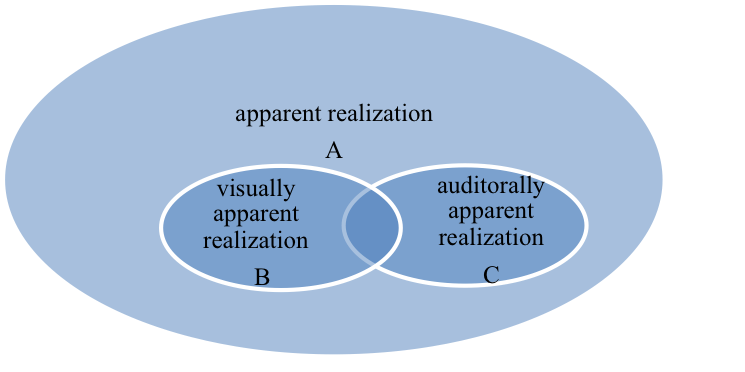
\includegraphics{napoli_fig1}
\caption{Entities of the world organized by type of
realization}
\label{fig:1}
\end{figure}

All iconic mappings between distinct entities rely on metaphor,
metaphony, and/or analogy, all filtered through experience, so all of
them are complex. However, some of the mappings are more complex than
others. With respect to Korean and Japanese mimetics, for example, we
can find mappings between a sound on the one hand and a taste or a mood
on the other \citep{garrigues1995,iwasaki2013}. That is, we have a
mapping between something in the area C and something in the area A−C.
So the mapping is cross-modal.

Iconic mappings in speech or sign into abstract meanings are necessarily
cross-modal since they are mapping between elements in B or C and
elements in A − (B ∪ C). Metaphor is the key mechanism used in sign
languages for this kind of conceptual mapping \citep{borghi2014}. Many
conceptual metaphors hold both in spoken and sign languages (Roush
2016).

Metaphoric mappings that cross perceptual modalities are labeled
synesthesia (Cytowic 1989, among many). We find mappings between many
different senses, where a given sense S\textsubscript{1} can elicit a
different sense S\textsubscript{2}, and vice-versa. For example, texture
can elicit visual forms \citep{simner2012,ludwig2013} and visual forms can elicit textures \citep{albertazzi2016}.

Many instances of synesthesia map a variety of senses onto auditory
forms. Thus the odors of perfumery are mapped onto pitches \citep{belkin1997} and food smells are mapped onto the sounds of musical
instruments \citep{crisinel2012}. Likewise, we find mappings from
a variety of senses onto visual forms. With regard to odor again,
\citet{dematte2006} examine odors mapped onto color hue, and \citet{kemp1997} show that intense smells are associated with darker
colors. \citet{hanson2013} look at the mappings
from odors onto visual shape entities, where intense, unpleasant odors
elicit angular shapes and other odors elicit rounded shapes.

Importantly, both hearing and deaf people can smile when a child says,
``This tastes green.'' In fact, congenitally blind people and
congenitally deaf people are sensitive to synesthesia, and in the same
ways as sighted, hearing people \citep{ittyerah1988}. A recent
study shows that color-shape associations, in particular, are consistent
across deaf and hearing people \citep{chen2014}. Further, sign
recognition involves reference to sensory-motor properties of one's own
body \citep{corina2016}, which would be compatible with sign
formation likewise involving such reference. In sum, there is every
reason to expect to find the effects of synesthesia in sign languages as
much as in spoken languages.

Cross-modal mappings can have multiple layers of complexity. Let's say
that we want to convey the sense of `happy' in a sign language. What
visual representation might we appeal to? A smile might come to mind.
And some languages use the smile, though they draw it (in a variety of
ways) rather than have the signer actually smile (such as the sign
languages of Italy, Latvia, Portugal, and Turkey). The problem with
using an actual smile is that that affective facial expression might
conflict with other information in the message. If we ask in a sign
language, ``Are you happy?'' we might well not smile, but use a neutral
mouth as other nonmanuals articulation (such as the eyebrows raising).
If we say in a sign language, ``I'm not happy,'' it might be odd to
smile (except in contrived circumstances). So the sense `happy' has to
be conveyed some other way. I conjecture that this way is through a
chain of mappings, a chain which necessarily has precisely two
cross-modal links -- one from an entity that has a somatosensory
realization other than visual to an entity that has a visual
realization, and the next from that visual entity to a third entity that
has a somatosensory realization other than visual (and see the
distinction between two types of icons in \citealt{pierce1932}). An iconicity
chain has complexity similar to that of the double metaphors of \citet{meir2010}, but iconicity chains are culture independent, since they are
grounded in biological properties.

In this regard, consider the sign \textsc{happy} in ASL in Figure 2.
(Figure from Lifeprint:
\url{http://www.lifeprint.com/asl101/pages-signs/h/happy.htm})


\begin{figure}
	\begin{tabularx}{\linewidth}{CCC}
		 \signpic{napoli_fig2a} & \signpic{napoli_fig2b} & \signpic{napoli_fig2c} \\
	\end{tabularx}
	\caption{\textsc{happy} in ASL}
	\label{fig:2}
\end{figure}

Here the hands hit the chest then circle away and hit again repeatedly.
My conjecture is that this sign is built on the fact that physical
activity correlates highly with happiness (Kahneman, Diener, and Schwarz
1999) and with a heartbeat that we are conscious of. So it's like our
heart is hopping inside our chests. The mapping is a chain from a
hopping heart (which we cannot see, but we can feel) to an external
representation of that heart (the visuals in Figure 2) and then to the
abstract meaning `happy'. So we are going from one somatosensory sense
to vision and then from vision to a sense that is an emotion. Both links
of the chain are cross-modal and both are iconic, as shown in Figure 3.

\begin{figure}
	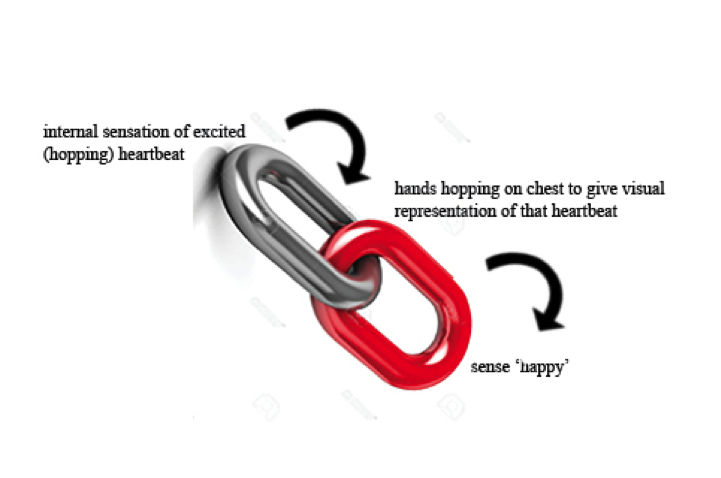
\includegraphics{napoli_fig3.png}
	\caption{Schema of the iconicity chain for \textsc{happy} in ASL}
	\label{fig:3}
\end{figure}

This iconicity chain between heart(beat) and happiness has its origins
in our biological selves; it digs down inside our bodies. As such, it is
culture-independent and we might expect to find sign languages using a
chest-touching sign for `happy' both among those that are genetically
related to or have had contact with ASL (as happens in the sign
languages of France and India) and among those that most likely
developed independently (as happens in the sign languages of Austria,
Germany, Iceland, and Sweden).

If we are alerted to likely possibilities for synesthesia in sign
languages -- that is, for iconicity chains -- not only might we find
them, but we might realize that signs we previously considered arbitrary
are not. I contend this not only because of my own initial examinations,
but because, on a theoretical basis, it should be true. Communication
systems are subject to two potentially conflicting pressures:
transmission efficiency, which drives them toward messages that are
simple to produce (and perceive), and comprehension efficiency, which
drives them toward messages that are semantically clear. As \citet[52]{roberts2015}) show in experimental work, ``where
iconicity was available, it provided scaffolding for the construction of
communication systems and was overwhelmingly adopted.'' This goes
hand-in-hand with work that shows that iconicity facilitates both
recognition and production of signs \citep{vinson2015}. In other
words, comprehension efficiency trumps transmission efficiency. Rightly
so. Non-arbitrary mappings, if they can be made, should be, since they
enhance interpretability (and see \citealt{givon1989}). To do otherwise would be
contrary to the overall goal of communication (and see \citealt{napoli-forthcoming}).

In the rest of this section I briefly mention two areas for research in
language synesthesia outside of speech, then focus on the area of
potential sources for iconicity chains in sign languages.

\subsection{Potential for iconicity chains in braille}

Blind hearing people can access speech easily, thus, generally, language
access is high, including access to all the mechanisms for synesthesia
that speech uses. However, language represented in print is visual, thus
inaccessible. The bumps in a braille cell allow print to be accessed
tactilely and, because of this, a range of possibilities for cross-modal
iconicity in language arise, where the connection between the two links
in the iconicity chain is a tactile entity (comparable to the visual
entity in sign language iconicity chains). So far as I know, such
possibilities are not well-explored, though the iconic possibilities in
rendering musical scores and literature on music theory are many \citep{pacun2009,johnson2009n}. Given that cutaneous perception is high, it's no
surprise that there's ongoing research on creating tactile icons
(tactons) that include rhythm, location, frequency, amplitude, and
duration of a tactile pulse, where iconicity influences the choices
designers are making on attaching meaning to the various tactile factors
\citep{brewster2004}, as well as V-Braille, a way to haptically
represent Braille characters on a touch screen (such as on a mobile
phone) \citep{jayant2010}.

\subsection{Potential for iconicity chains in tactile sign}

The deaf-blind cannot access language visually or aurally. Thus, another
area of exploration regarding synesthesia is tactile language for the
deaf-blind, a complex of methods, such as fingerspelling, on-body
signing, and hand-over-hand signing (\citealt{edwards2012}, and following).
Research has shown that visual and tactile iconicity ratings of signs
are similar across blind people, deaf people, and hearing-sighted
people, allowing indications of which signs should be most salient to
deaf-blind children \citep{griffith1983}.

\subsection{Potential for iconicity chains in sign languages}

Here I present the main course of this drawn-out feast in the form of a
sampling of cross-modal associations that could serve as fertile ground
for iconicity chains in sign languages. The iconic chains that interest
me below involve mappings from an entity that is not visually apparent
onto an entity that is visually apparent and then onto a meaning that is
not visual in nature. Thus both links in these iconic chains are
cross-modal. These are conceptually the most complex iconicity chains
and, thus, might be the hardest to recognize.

The growing literature on synesthesia includes mappings involving forms
that have realizations in various aspects of the somatosensory
experience, including texture, temperature, weight, taste, smell, shape,
emotions -- the sorts of things that many of the mimetics in Korean and
Japanese are based on. For humans, `meanings' associated with such
forms, as discussed in the literature cited below, tend to be general
and abstract rather than particular and concrete (to be contrasted with
the `meanings' such forms might convey to nonhumans). For example, with
respect to associations from a visual entity, a color might be
associated with a broadly understood emotion \citep{johnson1986}, and with respect to associations from an auditory entity,
pitch and tempo in music might be associated with a broadly understood
emotion \citep{hevner1937,brower2000}. Often the emotion is hedonic, since
the orbitofrontal cortex, which is involved in sensory integration, is
also involved in hedonic experience \citep{kringelbach2005}. Evoking such
general mappings has been claimed to be effective in psychopathology
therapies (\citealt{lang1979}, and much work since).

Let's look at five potential sources for iconic chains in sign
languages: mappings from texture, temperature, weight, taste, and smell.

\paragraph{Mappings from texture} Research on baby rhesus monkeys shows they
choose soft models of their mothers over wire ones \citep{harlow1959}, which
has been taken to show the importance of touch (particularly human
touch) for human babies \citep{lynch1970,schneider1996}. Further, neonates
in pain find comfort in skin-to-skin contact -- which introduces a
complex of factors, to be sure, but all transferred via that pliable
skin \citep{kostandy2008}. The potential, then, for an iconicity chain taking
us from some relevant touch to the visuals related to that touch and
then to the meaning `safety' or `love' arises. I believe that potential
is realized. The sign \textbf{\textsc{güvenli}} `safe' in the sign
language of Turkey uses two claw handshapes (the curled-5-handshape),
which rake across the chest out to each side, one above the other (shown
in the left side of Figure 4). This sign at first has no apparent
iconicity. However, the sign \textbf{\textsc{kürk}} `fur coat' is a
compound of the sign for `fur' and the sign for `coat'. The sign for
`fur' has two claw handshapes raking out to each side from the center of
the face (shown in the right side of Figure 4).

\begin{figure}
	\begin{tabularx}{\textwidth}{CC}
	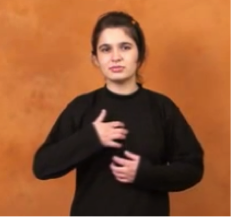
\includegraphics{napoli_fig4a} & 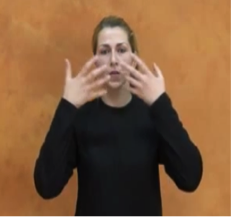
\includegraphics{napoli_fig4b}\\
	\end{tabularx}
\centering\caption{ `Safe' (left) and `fur' (right) in the sign language of
Turkey}
\label{fig:4}
\end{figure}

The signs differ only by the parameter of location: one is on the chest,
the other is on the face; one places one higher, the other has the hands
at the same level. I suggest the iconicity chain mapping from the
texture of softness onto the visual of fur or hair on the chest then
onto the feeling of security and coziness that juvenile mammals
(including humans) experience as they nestle against the chest of mature
mammals (including male humans; i.e., daddy keeps us safe).

\paragraph{Mappings from temperature} Research on human emotional responses
to changing a hand temperature show that changes of 6 degrees centigrade
are distinctly unpleasant \citep{salminen2013}. Thus one might
associate warmth with pleasure/health/life, but extreme heat or cold
with displeasure/fear/death. Consider here the sign \textsc{teama}
`fear' in the sign language of Romania. The arms are bent and held close
to the body, shaking them as if in a shiver (shown in the left side of
Figure 5 -- this is an embodiment sign, so the signer is shivering).
Certainly, humans shake not only when they experience cold (where
shivers occur because the drop in temperature signals the hypothalamus
to stimulate muscle contractions to warm up the body) but when they
experience fear (where adrenaline causes shivers) and a number of other
emotions. And the sign \textsc{strach} `fear' in the sign language of
Poland is also built on an image of shaking, but this time it's the legs
that shake (shown in the right side of Figure 5 -- this is a classifier
sign, so the dominant hand represents two legs that shake on the palm of
the nondominant hand).

\begin{figure}
	\begin{tabularx}{\textwidth}{CC}
		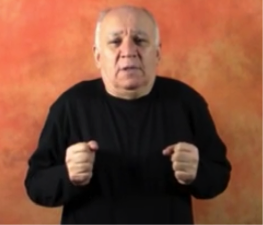
\includegraphics{napoli_fig5a} & 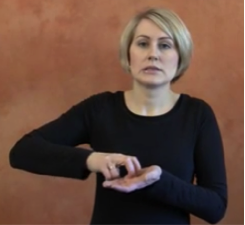
\includegraphics{napoli_fig5b}\\
	\end{tabularx}
	\caption{`Fear' in the sign languages of Romania (left) and Poland (right)}
	\label{fig:5}
\end{figure}

What makes me think the shaking is related directly to coldness in the
sign in Romania is that this sign is identical to the sign for `cold' in
many sign languages (such as the sign languages America, Austria,
Britain, Czech Republic, Estonia, Germany, India, Italy, Japan, Russia,
Spain, Turkey -- a group that has three families in it, but also several
languages that are independent from all others in that group). So the
iconicity chain in the sign language of Romania would go from the
sensation of coldness to the visually recognizable action of shivering
to the emotion of fear (and see discussion on spoken languages in this
regard in \citealt{atkins1995}).

\paragraph{Mappings from weight} There is little work in the literature
regarding synesthesia and weight, however some work suggests a
synesthetic link between weight and color brightness, where the darker a
color is, the heavier it is perceived to be \citep{ward2008}. Any iconic chain of this sort in a sign language would have only
one link being cross-modal.

Given my own experience with the world, however, I suspect other
iconicity chains regarding weight exist where both links are
cross-modal. For example, heavy might be associated with
strong/substantial and light might be associated with weak/insubstantial
in a broad range of contexts (such as judging food sources) while in
other contexts heavy might be associated with dangerous/overwhelming and
light with innocuous/possible (such as in lifting objects). My
speculations might find confirmation. The signs for `heavy' and `strong'
are close to identical to each other in the sign languages of Austria
and Germany (which might or might not be independent facts -- see \citealt{napolisanders}), where the visual image is related to lifting
something heavy. In Figure 6 we see the sign for `heavy' in Austria. In
Figure 7 we see the sign for `strong' in Austria. The handshapes and
locations are the same. The orientation of the palms is upward in
`heavy' and the movement is relatively slow. The orientation of the
palms is toward the signer in `strong' and the movement is rapid (which
is why the screenshot is blurred).

\begin{figure}
	\begin{tabularx}{\textwidth}{CC}
		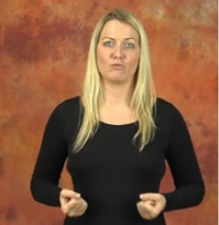
\includegraphics{napoli_fig6a} & 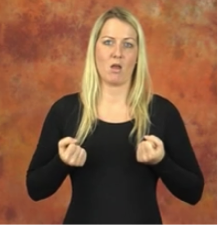
\includegraphics{napoli_fig6b}
	\end{tabularx}
	\caption{`Heavy' in the sign language of Austria}
	\label{fig:6}
\end{figure}

\begin{figure}
	\begin{tabularx}{\textwidth}{CC}
		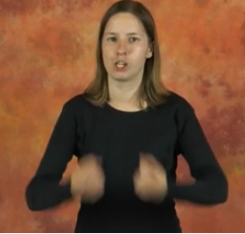
\includegraphics{napoli_fig7a} & 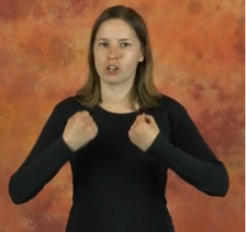
\includegraphics{napoli_fig7b}
	\end{tabularx}
	\caption{`Strong' in the sign language of Austria}
	\label{fig:7}
\end{figure}


Further, the signs for `lightweight' and `possible' are similar to one
another in the sign language of India.

\paragraph{Mappings from taste} It appears that humans are born with a
negative reaction (disgust) to acidic and a positive one to sweet (Fox
and Davidson 1986). The sweet response is to taste rather than to a
high-energy source, since neonates respond equally to sucrose as to
artificial sweeteners \citep{ramenghi1996}. The sign for `sweet' is
made at (or below or beside) the mouth in sign language after sign
language, as expected (the only exception on spreadthesign.com being the
sign language of Estonia, but it looks like the signer actually signed
the sense of `candy', rather than of the taste `sweet'). Perhaps the
association of sweetness with goodness is behind the fact that the sign
for `good' is made at the mouth in several languages (including those of
America, Brazil, France, and Italy -- all members of a single family).
Of course, the reason here could as easily be that food and eating in
general are associated with well-being (at least in that language
family).

\paragraph{Mappings from smell} Some odors elicit pleasure and some
displeasure \citep{alaoui1997}, which might mean `good/come
close' (the smell of a hot bowl of pasta) versus `bad/go away' (the
smell of a skunk). Recent work suggests that affective experiences
induced by odors are quite general, but allow for refinement of types,
involving ``well-being, social interaction, danger prevention, arousal
or relaxation sensations, and conscious recollection of emotional
memories'' \citep[49]{chrea2009}. Iconic chains mapping from odor to a
visual form to an emotion occur. The sign \textsc{repugnar} `disgust' in
the sign language of Brazil is clearly built on the perception of a bad
smell (and is similar to \textsc{chiero} `odor'), as is the sign
\textsc{asquear} `odor' in the sign language of Spain. In Figure 8 we
see the Brazil sign, where the hand moves to the nose, then out to the
ipsilateral side, then down and across to the contralateral side.

\begin{figure}
	\begin{tabularx}{\textwidth}{CCC}
		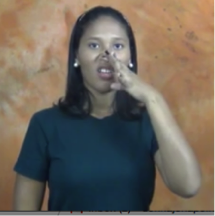
\includegraphics{napoli_fig8a} & 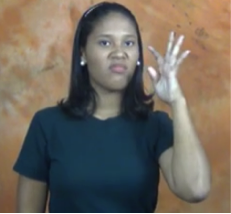
\includegraphics{napoli_fig8b} & 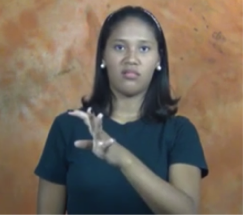
\includegraphics{napoli_fig8c}\\
	\end{tabularx}
	\caption{`Disgust' in the sign language of Brazil}
	\label{fig:8}
\end{figure}

\section{Conclusion }

Understanding iconicity in sign languages requires attention to
cross-modal associations, which might be complex -- involving an
iconicity chain that has two mappings, rather than one. Thus the present
work aims to alert researchers to such associations.

The benefits of a more (nearly) adequate approach to iconicity in
communication are several. Understanding iconicity can help separate out
what language is responsible for from what general communication is
responsible for, and it might help us understand some of the more thorny
areas in sign language studies, including why the signs for abstract
concepts can be similar in unrelated languages.

Of particular interest to me is how languages change over time.  Sign languages lack the regular changes typical of spoken language change (as discussed in any classical or more recent introduction to historical linguistics, such as \citealt{anttila1972}) but, instead, display only tendencies \citep{moser1990}.  Thus diachronic changes motivated by the drive for ease of articulation \citep{napoli2014n,sanders2016a,sanders2016b} apply erratically. The (near) insistence on maintaining iconicity might be at least partially responsible here, especially in light of the fact that iconic words in spoken language sometimes do not obey the same constraints that non-iconic words obey (as noted in \citealt{meir2010}).  For example, well-formedness conditions and ordinary phonological rules do not always apply to Japanese mimetics \citep{ito1995}.  And the onomatopoetic word \emph{peep} in English (\emph{pīpen} in Middle English) did not undergo the Great Vowel Shift perhaps because of the desire to maintain the [i] which connects to small size \citep[294]{hock1986}.  Additionally, in West Papuan languages it looks like onomatopoeia in words meaning ‘chicken’ and ‘cat’ may have contributed both to the spread of these words among genetically unrelated languages and to their resistance to phonological change over time \citep{gasser}. We find further evidence of onomatopoeia being ill-behaved in Italian (Marina Nespor, personal communication, December 2016).  The horse in Italian goes \emph{iiii} (that is [iiii], while the verb for this is unrelated:  nitrire), and many parents reading to small children might enunciate four syllables here.  But in the rest of the lexicon there are no words that contain a sequence of four uninterrupted vowels, except perhaps in other animal sounds.  For example, the goat or sheep might go [be], [bee], [beee], or [beeee] (while the verb for this is well-formed: \emph{belare}).   Likewise, the mouse goes [skwit skwit], but elsewhere in Italian words do not end in [t], nor do syllables unless the [t] is part of a geminate (and, again, the verb for this is well-formed: \emph{squittire}).  And in the Turkic language Kazakh, we find onomatopoeic words with consonant clusters that fall outside the range of normally attested clusters \citep{washington}.  In sum, iconicity allows an alignment between form and meaning, and the pressure to establish it when it is possible and the subsequent pressure to maintain it once it is established are strong.  


\printbibliography[heading=subbibliography,notkeyword=this]


\end{document}

